\section{Volume Estimation}
This section details the implementation of the chosen, SSP based volume estimation algorithm discussed in Section \ref{design:planimetry}. During this phase, several issues were overcome. \\

\subsection{How Many Planes?}
There was a necessary trade off between number of planes and quality of those planes. If the number of planes was too low, the volume estimation would be woefully inaccurate due to a lack of required granularity. If the number of planes was too high, then the volume would be inaccurate due to the lack of information contained within a plane. Sixty planes were chosen, based on a visual inspection of planes within the Corbett data set, shown in Figure \ref{fig:the_corbett_data_set}.\\

\begin{figure}[htb]
\begin{center}
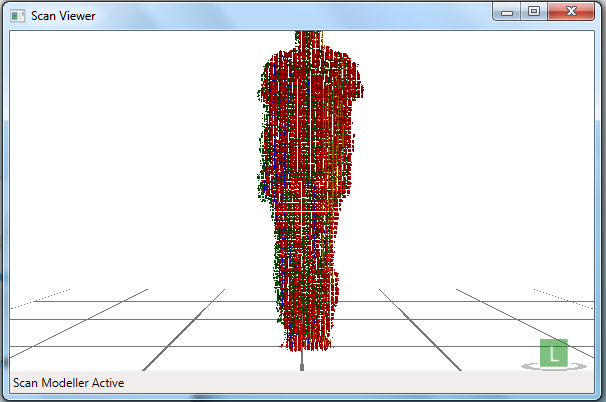
\includegraphics[scale=0.4]{images/corbett_dataset} 
\end{center}
\caption{The Corbett data set, stitched perfectly by the Bounding Box method}
\label{fig:the_corbett_data_set}
\end{figure}

\subsection{Noisy Data}
The data retrieved from the point clouds was not as originally expected. Firstly, the y-values were not discrete but continuous, as a result retrieving a plane at a single height would not result in ring of points. Therefore, a plane would be retrieved from a range of heights and then the points flattened to form a ring.\\

Also, the points were not close to a convex hull as expected, see Figure \ref{slice 30 from the corbett data set}, but were in fact quite noisy. As such, the points were \emph{sub-sampled} and then averaged to reduce noise. Sub-sampling by a factor of $n$ involved discarding $n-1$ points out of every $n$. Averaging points by a factor of $n$ involved adding the co-ordinate values of $n$ points, averaging them into a single point and returning a list of such average points. Figure \ref{plane 30 from the corbett data set sub-sampled and averaged} shows plane 30 of the Corbett data set after being sub-sampled and averaged by a factor of 7. A factor of 7 was chosen again based on visual inspection of the planes.\\

\begin{figure}[htb]
\begin{center}
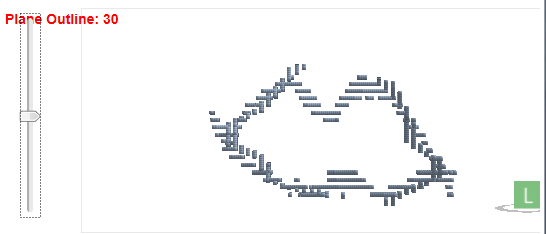
\includegraphics[scale=0.4]{images/notasexpected} 
\end{center}
\caption{Plane 30 from the Corbett data set}
\label{slice 30 from the corbett data set}
\end{figure} \\

\begin{figure}[htb]
\begin{center}
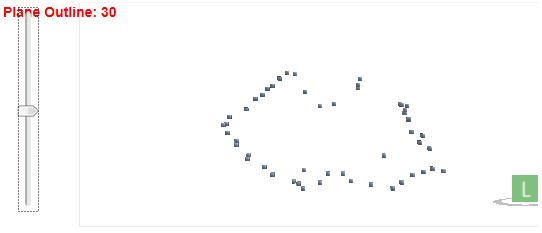
\includegraphics[scale=0.4]{images/improved} 
\end{center}
\caption{Plane 30 from the Corbett data set sub-sampled and averaged}
\label{plane 30 from the corbett data set sub-sampled and averaged}
\end{figure} \\

\subsection{The Need for a Transform Constant}
Early metrics returned were calculated in \emph{point cloud space} (PCS), as evidenced by the Corbett data subject's height being predicted as 2.27m. Therefore, a transform constant is required to move between measurements calculated in point cloud space (PCS) and measurements in terms of SI units in \emph{real world space} (RWS). Such a transform was believed necessary because the Kinect stores distances in terms of pixels and points, rather than meters and it is real world measurements that the calculated volume should be given. The transform was suspected to be multiplicative and as such is of the form shown in equation \ref{imp: transform between pcs and rws}. Determination of this constant was determined empirically during testing.\\

\begin{equation}
Volume_{PCS} * Transform Constant = Volume_{RWS}
\label{imp: transform between pcs and rws}
\end{equation}\\